% K5 and K3,3 with one crossing (generated by figs_c1ch07.py).
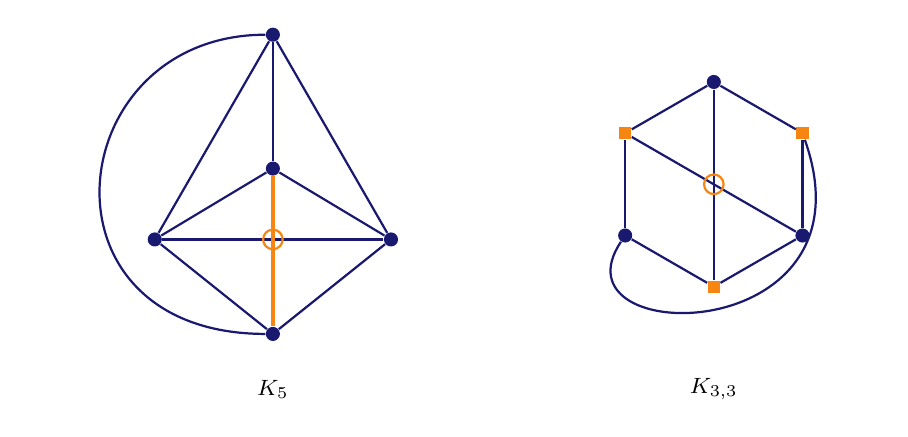
\begin{tikzpicture}[x=1cm,y=1cm,v/.style={circle,fill=MidnightBlue,inner sep=1.8pt},w/.style={rectangle,fill=BurntOrange,inner sep=2.2pt},e/.style={thick,MidnightBlue},l/.style={font=\footnotesize}]
\node[v] (A) at (0,0) {};
\node[v] (B) at (3,0) {};
\node[v] (C) at (1.5,2.6) {};
\node[v] (D) at (1.5,0.9) {};
\node[v] (E) at (1.5,-1.2) {};
\draw[e] (A) -- (B);
\draw[e] (B) -- (C);
\draw[e] (C) -- (A);
\draw[e] (D) -- (A);
\draw[e] (D) -- (B);
\draw[e] (D) -- (C);
\draw[e] (E) -- (A);
\draw[e] (E) -- (B);
\draw[e] (E) .. controls (-1.6,-1.2) and (-1.2,2.6) .. (C);
\draw[e,BurntOrange,very thick] (E) -- (D); \node[circle,draw=BurntOrange,thick,inner sep=2.5pt] at (1.5,0) {};
\node[l] at (1.5,-1.9) {$K_5$};
\node[v] (h0) at (7.100,2.000) {};
\node[w] (h1) at (5.974,1.350) {};
\node[v] (h2) at (5.974,0.050) {};
\node[w] (h3) at (7.100,-0.600) {};
\node[v] (h4) at (8.226,0.050) {};
\node[w] (h5) at (8.226,1.350) {};
\draw[e] (h0) -- (h1);
\draw[e] (h1) -- (h2);
\draw[e] (h2) -- (h3);
\draw[e] (h3) -- (h4);
\draw[e] (h4) -- (h5);
\draw[e] (h5) -- (h0);
\draw[e] (h0) -- (h3); \draw[e] (h1) -- (h4);
\draw[e] (h2) .. controls (5.00,-1.4) and (9.20,-1.4) .. (h5);
\node[circle,draw=BurntOrange,thick,inner sep=2.5pt] at (7.10,0.7) {};
\node[l] at (7.10,-1.9) {$K_{3,3}$};
\end{tikzpicture}
